\chapter{Parareal Method}
\label{sec:pr}

The parareal method is a parallel-in-time integration scheme to solve \acp{ODE}.
It goes back to \cite{Lions2001},
though the most common form also used in this thesis first appeared in \cite{Baffico2002}.
In this chapter we'll first describe the general properties of the parareal method,
and derive it as a Newton method following \cite{Gander2007}.
Then, in \autoref{sec:pr:DRE} we'll adapt the method for \acp{DRE}.
Lastly, in \autoref{sec:pr:alternatives} we'll briefly discuss alternative methods to parallelize matrix equations.

\section{General Properties}
\label{sec:pr:properties}

Consider the autonomous \ac{IVP}
\begin{equation}
  \label{eq:IVP}
  \left\{
  \begin{aligned}
    \dot u &= f \circ u \\
    u(t_0) &= u_0
  \end{aligned}
  \right.
\end{equation}
over the time span $[t_0, t_f]$.
Fix a discretization $t_0 < t_1 < \ldots < t_N = t_f$,
let $F$ denote a fine/high-precision solver of the \ac{IVP} above,
$F(t, t_0, u_0) \approx u(t)$,
and $G$ a coarse/lower-precision one.
Then the parareal method to compute $U_n \approx u(t_n)$ reads
\begin{equation}
  \label{eq:pr:method}
  \left\{
  \begin{aligned}
    U^0_{n+1} &:= G(U^0_n) \\
    U^{k+1}_{n+1} &:= G(U^{k+1}_n) + F(U^k_n) - G(U^k_n)
  \end{aligned}
  \right.
\end{equation}
where $U^0_0 := u_0$ and $G(U_n) := G(t_{n+1}, t_n, U_n)$
integrates from $t_n$ to $t_{n+1}$,
and similarly does $F$.

\begin{proposition}[Diagonal Convergence]
\label{thm:pr:conv}
  Stage $n$ of the parareal method converges after at most $n$ iterations:
  \begin{equation*}
    U^k_n = U^n_n = F(U^{n-1}_{n-1})
    \quad
    \forall k \geq n
  \end{equation*}
\end{proposition}
\begin{proof}
  Due to $U^k_0 = u_0$ for all $k$,
  it follows by induction $\forall k \geq n$:
  \begin{equation*}
    \begin{array}{r@{}l@{}l@{}l}
      U^{k+1}_{n+1}
      :={} & F(U^k_n) &{}+ G(U^{k+1}_n) &{}- G(U^k_n) \\
      ={}  & F(U^n_n) &{}+ G(U^n_n)     &{}- G(U^n_n)
      = F(U^n_n)
    \end{array}
  \end{equation*}
\end{proof}

This will become handy for the implementation.
In particular, note that if stage $n$ of the parareal method converged,
\ie $U^{k+1}_n \approx U^k_n$,
stage $n+1$ will converge after the same iteration:
\begin{equation}
  \begin{array}{r@{}l@{}l@{}l}
    U^{k+1}_{n+1}
    :={}      & F(U^k_n) &{}+ G(U^{k+1}_n) &{}- G(U^k_n) \\
    \approx{} & F(U^k_n) &{}+ G(U^k_n)     &{}- G(U^k_n)
    = F(U^k_n)
  \end{array}
\end{equation}
Therefore,
assuming $G$ is well conditioned,
there is no need to compute $G(U^{k+1}_n)$.

\begin{figure}[t]
  \centering
  \begin{tikzpicture}[
  text height=1.5ex,
  text depth=0.25ex,
]
  \graph[
    math nodes,
    grow right=2cm,
    diag/.style={bend left, shorten >=2pt},
  ]{
    Unk/"U_{n-1}^{k-1}" [label=above:$\vdots$]
    -> Gnk/"G(U_{n-1}^{k-1})" -> Un1k/"U_{n}^{k-1}" [label=above:$\vdots$]
    -> Gn1k/"G(U_{n}^{k-1})" -> Un2k/"U_{n+1}^{k-1}" [label=above:$\vdots$],
    "" -!- Fnk/"F(U_{n-1}^{k-1})" -!- "" -!- Fn1k/"F(U_{n}^{k-1})",
    Unk1/"U_{n-1}^{k}"
    -> Gnk1/"G(U_{n-1}^{k})" -> Un1k1/"U_{n}^{k}"
    -> Gn1k1/"G(U_{n}^{k})" -> Un2k1/"U_{n+1}^{k}",
    "" -!- Fnk1/"F(U_{n-1}^{k})" -!- "" -!- Fn1k1/"F(U_{n}^{k})",
    Unk2/"U_{n-1}^{k+1}" [label=below:$\vdots$]
    -> Gnk2/"G(U_{n-1}^{k+1})" -> Un1k2/"U_{n}^{k+1}" [label=below:$\vdots$]
    -> Gn1k2/"G(U_{n}^{k+1})" -> Un2k2/"U_{n+1}^{k+1}" [label=below:$\vdots$];

    Unk -> Fnk -> Un1k1 -> Fn1k1 -> Un2k2;
    Un1k -> Fn1k -> Un2k1;
    Unk1 -> Fnk1 -> Un1k2;
    Gnk -> [diag] Un1k1;
    Gnk1 -> [diag] Un1k2;
    Gn1k -> [diag] Un2k1;
    Gn1k1 -> [diag] Un2k2;
  };
  \node [left=5mm of Unk.center] {$\cdots$};
  \node [left=5mm of Unk1.center] {$\cdots$};
  \node [left=5mm of Unk2.center] {$\cdots$};
  \node [right=5mm of Un2k.center] {$\cdots$};
  \node [right=5mm of Un2k1.center] {$\cdots$};
  \node [right=5mm of Un2k2.center] {$\cdots$};
\end{tikzpicture}

  \caption{Dependencies between parareal values $U^{k+1}_{n+1}$}
  \label{fig:pr:DAG}
\end{figure}

\todo[inline]{Add DAG of beginning of early parareal stages: $U_0^0,\ldots,U_2^2$}

Note how $G(U_n^{k+1})$ is needed twice.
Therefore, a reasonable scheduling pattern that exploits good data locality is the following:
\begin{equation}
  \text{stage $n+1$:}
  \quad
  %TODO: arrows     //
  \ldots, G(U_n^k), U_{n+1}^{k+1}, F(U_n^{k+1}), \ldots
  %        //
\end{equation}

\begin{example}[Linear \acs*{ODE}]
  Let $\phi := \frac{1+\sqrt{5}}{2}$ denote the golden ratio and
  let $\kappa := \frac{2}{\pi} \log \phi$.
  Consider the \ac{IVP}
  \begin{equation}
    \label{eq:pr:linear}
    \left\{
    \begin{aligned}
      \dot u &= \begin{bmatrix}
        \kappa & -1 \\
        1 & \kappa
      \end{bmatrix} u \\
      u(0) &= \begin{bmatrix}
        -1 \\ -\kappa
      \end{bmatrix}
    \end{aligned}
    \right.
  \end{equation}
  for $t\in[0,2\pi]$.
  Let $N := 5$, $\tau := 2\pi/N$, and $t_n := n\tau$ for $n\in\Set{0,\ldots,N}$.
  Further, let $F$ and $G$ be implicit Euler schemes using step sizes $\tau/100$ and $\tau$, respectively.
  If the fine solver internally uses a finer mesh,
  by \autoref{thm:pr:conv},
  the global solution $x$ may be retrieved at that fine resolution $\tau/100$.

  \begin{figure}[tb]
    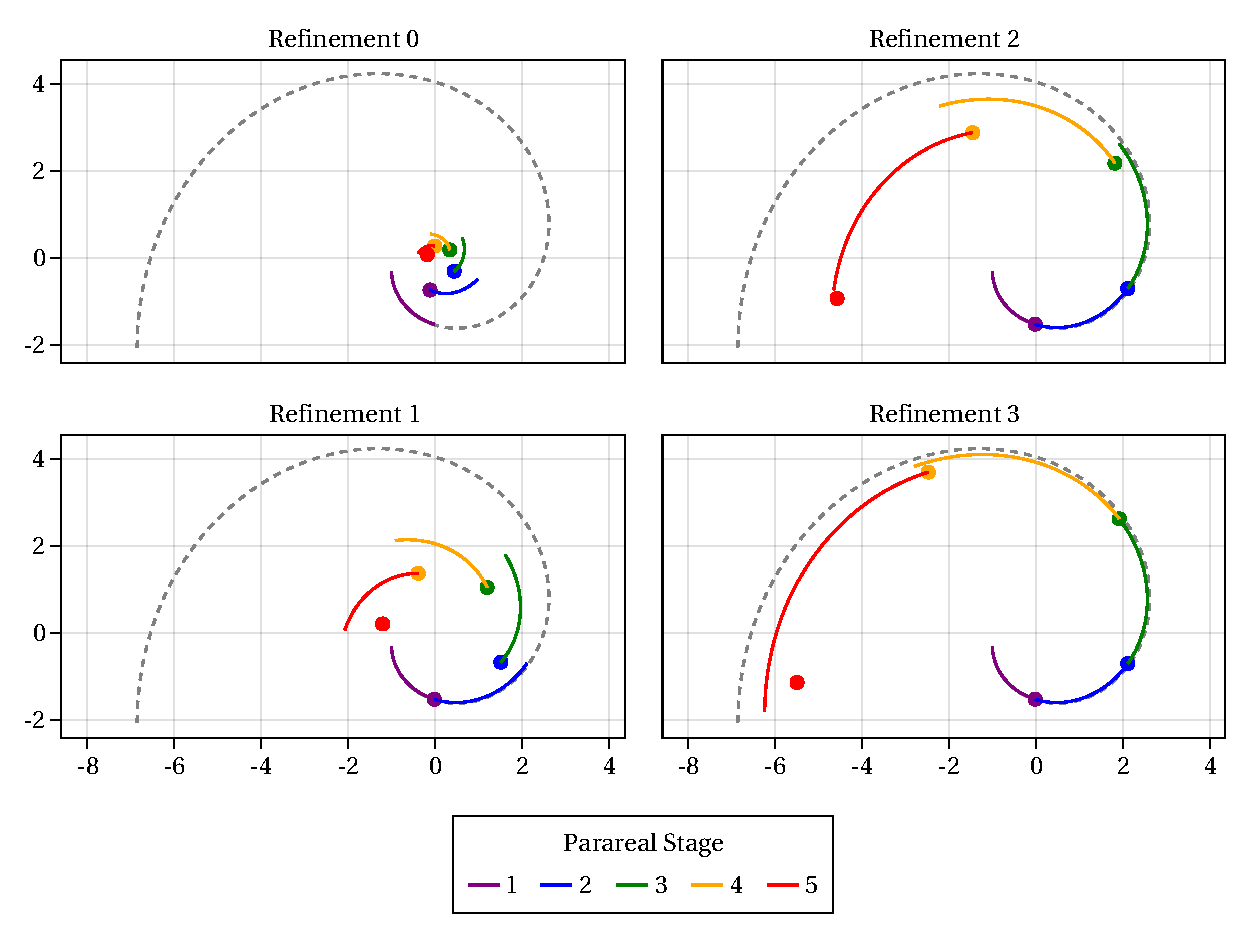
\includegraphics[width=\textwidth]{figures/fig_parareal_example.pdf}
    \caption[Parareal method applied to a linear ODE]{%
      First couple of refinements $k$ of the
      parareal method applied to the linear problem \eqref{eq:pr:linear}.
      The stages $n$ are decoded by color,
      dots denoting $U^k_n$ and lines $F(\optional{}, t_{n-1}, U^k_{n-1})$.
      The gray curve represents the exact solution.
    }
    \label{fig:pr:linear}
  \end{figure}

  \autoref{fig:pr:linear} shows the first couple of iterations of the parareal method applied the problem above.
  For a fixed refinement $k$,
  the values $U^k_n \approx u(t_n)$ (represented by dots) are computed in sequence,
  \cf the horizontal traces in \autoref{fig:pr:DAG}.
  After that, the fine solutions $F(U_n^k)$ (represented by lines) can then be computed in parallel.
  The parareal method only ensures convergence of $U_n^k$.
  Therefore, before convergence is reached,
  the high-resolution trajectories are discontinues at $t_n$.
  Furthermore, note that the overall accuracy of the parareal solution is limited by the accuracy of $F$,
  which explains the remaining gap between the colored and the gray line.
\end{example}

The parareal method may be seen \eg as a deferred correction method,
a special case of multiple shooting, or a Newton method.

\section{Parareal as a Special Case of Multiple Shooting}
\label{sec:pr:newton}

Consider the autonomous \ac{IVP}
\begin{equation}
  \label{eq:IVP}
  \left\{
  \begin{aligned}
    \dot u &= f \circ u \\
    u(t_0) &= u_0
  \end{aligned}
  \right.
\end{equation}
Note that the solution $u : [t_0,t_N] \to V $ depends on the initial value $U_0$.
For a discretization $t_0 < t_1 < \ldots < t_N$
define the local problems
\begin{equation}
  \left\{
  \begin{aligned}
    \dot u_i &= f \circ u_i \\
    u_i(t_i) &= U_i
  \end{aligned}
  \right.
\end{equation}
for $i \in \Set{0,\ldots,N-1}$
and determine suitable initial values $U_i$.
Watch the slight abuse of notation for the initial value $u_0 \in V$ and the solution to the local problem $u_0 : [t_0,t_1] \to V$.
The local solutions $u_i : [t_i,t_{i+1}] \to V$ represent a global solution to \eqref{eq:IVP} if
\begin{equation}
  F(U_0, \ldots, U_{N-1}) :=
  \left(
  \begin{aligned}
    U_0 &- u_0 \\
    U_1 &- u_0(t_1) \\
    &\vdotswithin{-} \\
    U_{N-1} &- u_{N-2}(t_{N-1})
  \end{aligned}
  \right)
  \overset{!}{=} 0.
\end{equation}
Let $U := (U_0, \ldots, U_{N-1})$ and $\mathcal J_F(U)$ denote the Jacobian of $F$ at $U$.
Then, Newton's method reads
\begin{equation}
  U^{k+1} = U^k - \mathop{\mathcal J_F(U^k)^{-1}} F(U^k)
\end{equation}
or, equivalently, avoiding the inversion of the Jacobian,
\begin{equation}
  \begin{pmatrix}
    I \\
    -\pdiff{U_0}{u_0}(t_1, U_0) & I \\
    & \ddots & \ddots \\
    && -\pdiff{U_{N-2}}{u_{N-2}}(t_{N-1}, U_{N-2}) & I
  \end{pmatrix}
  (U^{k+1} - U^k) = -F(U^k)
\end{equation}
Writing the above in separate equations yields
\begin{equation}
  \left\{
  \begin{aligned}
    U^{k+1}_0 &= u_0 \\
    U^{k+1}_i &= u_i(t_{i+1}, U^k_n) + \pdiff{U^k_i}{u_i}(t_{i+1}, U^k_i) (U^{k+1}_i - U^k_i).
  \end{aligned}
  \right.
\end{equation}
Lastly, choosing a fine propagator $F(U^k_i) := F(t_{i+1}; t_i, U^k_i) \approx u_i(t_{i+1}, U^k_i)$,
a coarse propagator $G$ according to
\begin{equation}
  \label{eq:pr:G}
  G(U^{k+1}_i) - G(U^k_i)
  \approx
  \pdiff{U^k_i}{u_i}(t_{i+1}, U^k_i) (U^{k+1}_i - U^k_i)
\end{equation}
as well as initial values $ U^0_{i+1} = G(U^0_i) $
reveals the parareal method of \cite{Baffico2002}:
\begin{equation}
  \left\{
  \begin{aligned}
    U^0_{i+1} &= G(U^0_i),
    \quad
    U^0_0 = u_0 \\
    U^{k+1}_{i+1} &= F(U^k_i) + G(U^{k+1}_i) - G(U^k_i)
  \end{aligned}
  \right.
\end{equation}
A Taylor expansion of $G(U^{k+1}_i) \approx u_i(t_{i+1}, U^{k+1}_i)$ around $G(U^k_i)$ justifies \eqref{eq:pr:G}.

\section{Application to \act{DRE}s}
\label{sec:pr:DRE}

\todo[inline]{Formulate parareal update \wrt low-rank factorization $LDL^\T$}

Let the \acp{LRSIF}
\begin{equation}
\begin{aligned}
  G(X^{k+1}_i) &= \mathop{L_{G,k+1}} \mathop{D_{G,k+1}} \mathop{L_{G,k+1}^\T} \\
  F(X^k_i)     &= \mathop{L_{F,k}}   \mathop{D_{F,k}}   \mathop{L_{F,k}^\T} \\
  G(X^k_i)     &= \mathop{L_{G,k}}   \mathop{D_{G,k}}   \mathop{L_{G,k}^\T}
\end{aligned}
\end{equation}
be given.
Using the low-rank update formulas described in \autoref{sec:lowrank},
the parareal update of \eqref{eq:pr:method} reads
\begin{equation}
  \hat L \hat D \hat L^\T :=
  \begin{pmatrix}
    L_{G,k+1} &
    L_{F,k} &
    L_{G,k}
  \end{pmatrix}
  \begin{pmatrix}
    D_{G,k+1} \\
    & D_{F,k} \\
    && -D_{G,k}
  \end{pmatrix}
  \begin{pmatrix}
    L_{G,k+1}^\T \\
    L_{F,k}^\T \\
    L_{G,k}^\T
  \end{pmatrix}
  .
\end{equation}
Note the downdate in the last block component.
The actual low-rank representation of $X^{k+1}_{i+1}$ is set to a column compression of $\hat L \hat D \hat L^\T$
using \autoref{alg:lowrank:compression},
\begin{equation}
  X^{k+1}_{i+1}
  := LDL^\T
  :\approx \hat L \hat D \hat L^\T
  .
\end{equation}

\todo[inline]{%
Due to \autoref{thm:basics:dre-limit-are},
later parareal stages will require fewer Newton refinements
(than earlier stages) to reach convergence.}

\section{Alternative Parallel-in-Time Solvers}
\label{sec:pr:alternatives}
